% SC1007 — Chapter 3: Trees & Traversals
% No \documentclass — included by modules/SC1007/main.tex (book class).
\chapter{Trees \& Traversals}
\label{ch:trees-traversals}

\begin{quote}
\emph{``A tree is a hierarchy you can walk without getting lost.''} --- Traversals turn branching structure into linear order.
\end{quote}

\noindent\textbf{Prerequisites:} Ch.~1--2 (pointers, recursion, stack/queue). This chapter is the foundation for all search trees (Ch.~4--5) and graph traversals (Ch.~7).

\section*{Learning Outcomes}
After this chapter you will be able to:
\begin{enumerate}[label=(L\arabic*)]
    \item define trees, binary trees, height/depth and prove $n$ nodes $\to$ $n-1$ edges;
    \item implement the three DFS traversals (pre/in/postorder) recursively and iteratively;
    \item perform level-order (BFS) traversal and relate it to queues;
    \item reconstruct a binary tree from traversal pairs and analyse $O(n)$ costs.
\end{enumerate}

% ============================================================
\section{Tree Terminology}
\label{sec:tree-terms}
A \emph{tree} is a connected acyclic graph. A \emph{rooted tree} designates one node as root; every other node has a unique parent. A \emph{binary tree} gives each node at most two children: \texttt{left} and \texttt{right} (order matters).

For node $v$: \emph{depth} $=$ edges from root to $v$; \emph{height} $=$ longest downward path to a leaf. Height of tree $=$ height of root. Height of single-node tree $=0$; empty tree $=-1$ by convention.

\begin{theorem}
A tree with $n$ nodes has exactly $n-1$ edges. A binary tree of height $h$ has at most $2^{h+1}-1$ nodes.
\end{theorem}

\begin{figure}[h]
\centering
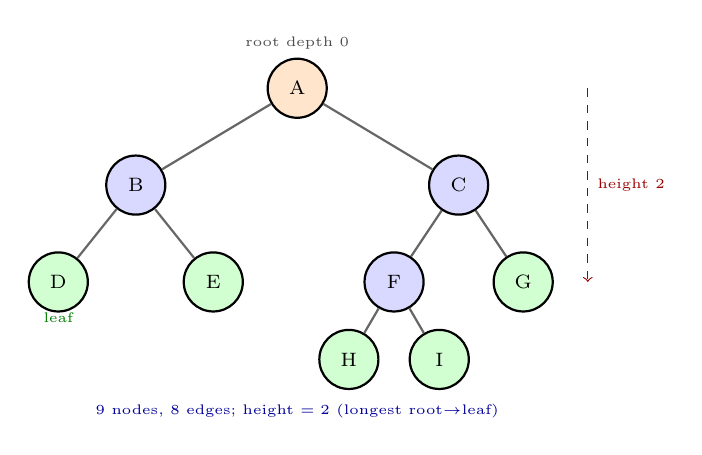
\begin{tikzpicture}[scale=0.82, every node/.style={font=\scriptsize},
  tnode/.style={circle, draw, thick, fill=blue!15, minimum size=0.75cm, inner sep=1pt},
  leaf/.style={circle, draw, thick, fill=green!18, minimum size=0.75cm, inner sep=1pt},
  edge/.style={thick, black!60}]
  \node[tnode, fill=orange!20] (r) at (4,3) {A};
  \node[tnode] (b) at (1.5,1.5) {B};
  \node[tnode] (c) at (6.5,1.5) {C};
  \node[leaf] (d) at (0.3,0) {D};
  \node[leaf] (e) at (2.7,0) {E};
  \node[tnode] (f) at (5.5,0) {F};
  \node[leaf] (g) at (7.5,0) {G};
  \node[leaf] (h) at (4.8, -1.2) {H};
  \node[leaf] (i) at (6.2, -1.2) {I};
  \draw[edge] (r) -- (b); \draw[edge] (r) -- (c);
  \draw[edge] (b) -- (d); \draw[edge] (b) -- (e);
  \draw[edge] (c) -- (f); \draw[edge] (c) -- (g);
  \draw[edge] (f) -- (h); \draw[edge] (f) -- (i);
  \node[font=\tiny, gray!60!black] at (4,3.7) {root depth 0};
  \node[font=\tiny, green!50!black] at (0.3,-0.55) {leaf};
  \draw[->, dashed, red!60!black] (8.5,3) -- (8.5,0) node[midway, right, font=\tiny] {height 2};
  \node[font=\tiny, blue!60!black] at (4,-2.0) {9 nodes, 8 edges; height $=2$ (longest root$\to$leaf)};
\end{tikzpicture}
\caption{A rooted binary tree. Orange = root, blue = internal, green = leaves. Depth and height illustrated.}
\label{fig:binary-tree}
\end{figure}

Storage: each node holds \texttt{val}, \texttt{left}, \texttt{right} pointers. Array embedding (heap-style, Ch.~5) stores node $i$'s children at $2i,2i+1$.

% ============================================================
\section{Depth-First Traversals}
\label{sec:dfs-traversals}
DFS visits recursively; three orders differ only in when the root is processed:

\begin{align}
\text{Preorder: }  &\text{root} \to \text{left} \to \text{right} \nonumber\\
\text{Inorder: }   &\text{left} \to \text{root} \to \text{right} \nonumber\\
\text{Postorder: } &\text{left} \to \text{right} \to \text{root} \nonumber
\end{align}

\begin{figure}[h]
\centering
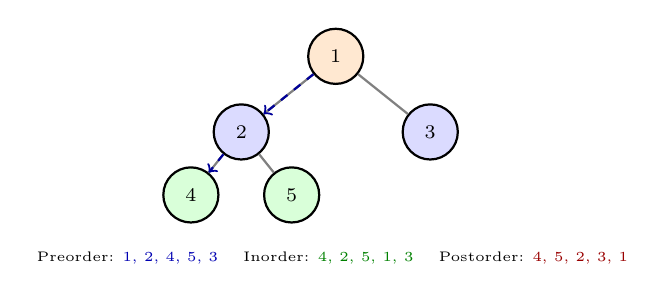
\begin{tikzpicture}[scale=0.80, every node/.style={font=\scriptsize},
  tnode/.style={circle, draw, thick, fill=blue!14, minimum size=0.70cm},
  edge/.style={thick, black!50}]
  % Small tree:     1
  %                / \
  %               2   3
  %              / \
  %             4   5
  \node[tnode, fill=orange!18] (1) at (3,2.2) {1};
  \node[tnode] (2) at (1.5,1.0) {2};
  \node[tnode] (3) at (4.5,1.0) {3};
  \node[tnode, fill=green!15] (4) at (0.7,0) {4};
  \node[tnode, fill=green!15] (5) at (2.3,0) {5};
  \draw[edge] (1)--(2); \draw[edge] (1)--(3); \draw[edge] (2)--(4); \draw[edge] (2)--(5);
  % Traversal orders below
  \node[font=\tiny, align=left] at (3,-1.0) {
    Preorder:  \textcolor{blue!70!black}{1, 2, 4, 5, 3} \quad
    Inorder:   \textcolor{green!50!black}{4, 2, 5, 1, 3} \quad
    Postorder: \textcolor{red!60!black}{4, 5, 2, 3, 1}
  };
  % Colored visit order arrows for preorder
  \draw[->, blue!60!black, thick, dashed] (1) -- (2);
  \draw[->, blue!60!black, thick, dashed] (2) -- (4);
\end{tikzpicture}
\caption{Five-node example with all three DFS orders. Preorder is used to copy; postorder to delete; inorder gives sorted order for BSTs (Ch.~4).}
\label{fig:traversal-orders}
\end{figure}

\begin{lstlisting}[language=Python]
# Recursive traversals -- O(n) time, O(h) stack space
def preorder(root):
    if not root: return
    visit(root)              # root first
    preorder(root.left)
    preorder(root.right)

def inorder(root):
    if not root: return
    inorder(root.left)
    visit(root)              # root in middle
    inorder(root.right)

def postorder(root):
    if not root: return
    postorder(root.left)
    postorder(root.right)
    visit(root)              # root last

# Iterative preorder with explicit stack
def preorder_iter(root):
    stack = [root] if root else []
    while stack:
        v = stack.pop()
        visit(v)
        if v.right: stack.append(v.right)
        if v.left:  stack.append(v.left)
\end{lstlisting}

Each node is visited once, each edge traversed twice (down and up): $\Theta(n)$ time, $\Theta(h)$ stack space ($\Theta(n)$ worst case for a chain, $\Theta(\log n)$ for balanced).

% ============================================================
\section{Level Order (BFS)}
\label{sec:level-order}
Level order visits nodes breadth-first using a queue:

\begin{lstlisting}[language=Python]
from collections import deque
def level_order(root):
    if not root: return
    q = deque([root])
    while q:
        v = q.popleft()
        visit(v)
        if v.left:  q.append(v.left)
        if v.right: q.append(v.right)
\end{lstlisting}

\begin{figure}[h]
\centering
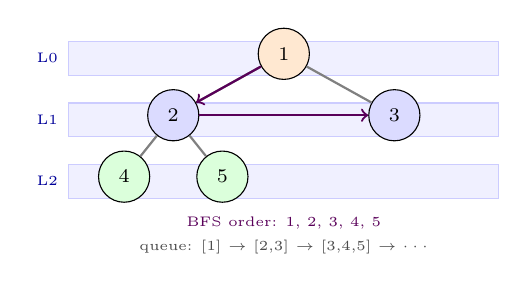
\begin{tikzpicture}[scale=0.78, every node/.style={font=\scriptsize}]
  % Levels
  \foreach \y/\lbl in {2.5/L0,1.5/L1,0.5/L2} {
    \draw[fill=blue!6, draw=blue!20] (-0.5,\y-0.35) rectangle ++(7.0,0.55);
    \node[font=\tiny, blue!60!black] at (-0.85,\y-0.07) {\lbl};
  }
  \node[circle, draw, fill=orange!18, minimum size=0.65cm] (1) at (3,2.5) {1};
  \node[circle, draw, fill=blue!14, minimum size=0.65cm] (2) at (1.2,1.5) {2};
  \node[circle, draw, fill=blue!14, minimum size=0.65cm] (3) at (4.8,1.5) {3};
  \node[circle, draw, fill=green!14, minimum size=0.65cm] (4) at (0.4,0.5) {4};
  \node[circle, draw, fill=green!14, minimum size=0.65cm] (5) at (2.0,0.5) {5};
  \draw[thick, black!50] (1)--(2); \draw[thick, black!50] (1)--(3);
  \draw[thick, black!50] (2)--(4); \draw[thick, black!50] (2)--(5);
  \draw[->, thick, violet!70!black] (1) -- (2);
  \draw[->, thick, violet!70!black] (2) -- (3);
  \node[font=\tiny, violet!70!black] at (3,-0.25) {BFS order: 1, 2, 3, 4, 5};
  \node[font=\tiny, gray!60!black] at (3,-0.65) {queue: [1] $\to$ [2,3] $\to$ [3,4,5] $\to\cdots$};
\end{tikzpicture}
\caption{Level-order traversal processes level $d$ before $d+1$. Queue holds the frontier.}
\label{fig:level-order}
\end{figure}

% ============================================================
\section{Reconstruction}
Given inorder $+$ preorder (or inorder $+$ postorder) the tree is uniquely determined. Preorder gives root first; inorder splits left/right subtrees. $O(n)$ with a hash map from value to inorder index. Preorder $+$ postorder alone is ambiguous for general binary trees.

% ============================================================

% --- Additional: Properties and threaded trees ---
\section{Tree Properties \& Variations}
\label{sec:tree-properties}
\textbf{Full / complete / perfect.} Full: every node has 0 or 2 children. Complete: all levels full except last, filled left-to-right (heap shape, Ch.~5). Perfect: all leaves at same depth, $n=2^{h+1}-1$.

\textbf{Threaded trees.} Replace null child pointers with threads to inorder successor/predecessor, enabling $O(1)$-space inorder without stack.

\textbf{Expression trees.} Leaves are operands, internal nodes operators. Inorder with parentheses recovers infix; preorder gives prefix (Polish); postorder gives postfix --- directly linking traversals to Ch.~2 evaluation.

\begin{lstlisting}[language=Python]
# Iterative inorder -- O(n) time, O(h) space, no recursion
def inorder_iter(root):
    stack, cur, out = [], root, []
    while stack or cur:
        while cur:
            stack.append(cur); cur = cur.left
        cur = stack.pop()
        out.append(cur.val)
        cur = cur.right
    return out
\end{lstlisting}

\section{Chapter Notes}
CLRS Ch.~10.4, 12. Weiss Ch.~4. DFS $\leftrightarrow$ stack, BFS $\leftrightarrow$ queue duality previews Ch.~7 graphs.

% ============================================================
\section{Exercises}
\label{sec:ch03-exercises}
\begin{enumerate}[label=E3.\arabic*, leftmargin=*, itemsep=0.7em]
    \item \textbf{Orders.} For the tree in Fig.~\ref{fig:binary-tree}, list preorder, inorder, postorder, and level order.
    \item \textbf{Iterative inorder.} Give an $O(n)$ iterative inorder using one stack (no recursion). Prove it visits nodes in inorder and uses $O(h)$ space.
    \item \textbf{Reconstruction.} Preorder $=[3,9,20,15,7]$, inorder $=[9,3,15,20,7]$. Reconstruct the tree and give its postorder. Explain the $O(n)$ hash-map algorithm.
    \item \textbf{Height vs.\ nodes.} Prove: a binary tree with $n$ nodes has height $h\ge\lceil\log_{2}(n+1)\rceil-1$, with equality for perfect trees. Give an example where $h=n-1$.
    \item \textbf{Expression tree.} Build the tree for $(3+4)\times(5-2)$ and show that preorder/postorder/inorder give prefix/postfix/infix notation. Which needs parentheses?
\end{enumerate}
% End of Chapter 3
